\documentclass[a4paper, 11pt]{article}
\usepackage{a4wide}
\usepackage[english]{babel}
\usepackage[T1]{fontenc}
\usepackage[utf8]{inputenc}
\usepackage{times}
\usepackage{ifthen}
\usepackage[sorting=none,backend=bibtex]{biblatex}
\addbibresource{bib.bib}
\usepackage{graphicx}
\graphicspath{{./images/}}
\DeclareGraphicsExtensions{.pdf,.jpeg,.png,.svg}
\usepackage{hyperref}
\usepackage{movie15}
\usepackage{fixltx2e}
\usepackage{amsmath}
\usepackage{amssymb}
\usepackage{nccmath}
\usepackage{csquotes}

\usepackage{color}
\usepackage{graphicx}
\usepackage{blindtext}
\usepackage{color}
\topmargin 0cm \textheight 23cm \parindent0cm

% ---------------------------------------------
%	Commands definition
% ---------------------------------------------
\newcommand{\R}{\mathbb{R}}

\newcommand{\myName}{Kandhasamy Rajasekaran}
\newcommand{\emailID}{kandhasamy@uni-koblenz.de}
\newcommand{\matriculationID}{216100855}

\newcommand{\Title}{Deep Learning techniques applied to Constituency Parsing of German}
\newcommand{\StartDate}{01-Aug-2019}
\newcommand{\EndDate}{31-Jan-2019}
\newcommand{\subject}{Institute f\"{u}r ComputerVisualistik}
%\newcommand{\expert}{Prof. Dr. Karin Harbusch}%inkl. Titel
\newcommand{\supervisor}{Prof. Dr. Karin Harbusch} %inkl. Titel
\newcommand{\secondSupervisor}{Denis Memmesheimer} %inkl. Titel
\newcommand{\type}{Master Thesis}
\begin{document}
% ---------------------------------------------
%	Title
% ---------------------------------------------
Universit\"{a}t Koblenz - Landau \hfill \today

Department f\"{u}r Informatik,

\subject{}

\supervisor{}

\secondSupervisor{}

\begin{center}
	\large{\bf \type{}  \myName{}}

	\vspace*{0.5cm}

	\large{\bf \Title}
\end{center}

\setlength{\parskip}{1.5ex plus0.5ex minus 0.5ex}

\selectlanguage{english}

\section{Introduction}
\frenchspacing

% Parsing - what is the purpose of doing it?
% How and where is it useful in NLP and other applications
% state an example
Constituency or Syntactic parsing is the process of determining the syntactic structure of a sentence by analysing its words based on underlying grammar. Constituency parsing is very important in natural language processing (NLP) because it plays a substantial role in mediating between linguistic expression and meaning \parencite*{Socher}. 

Say for e.g. the sentence 'Hans ißt die Äpfel' along with parts of speech (POS) tags, the parse tree is as follows:

\begin{figure}[htpb]
    \centering
    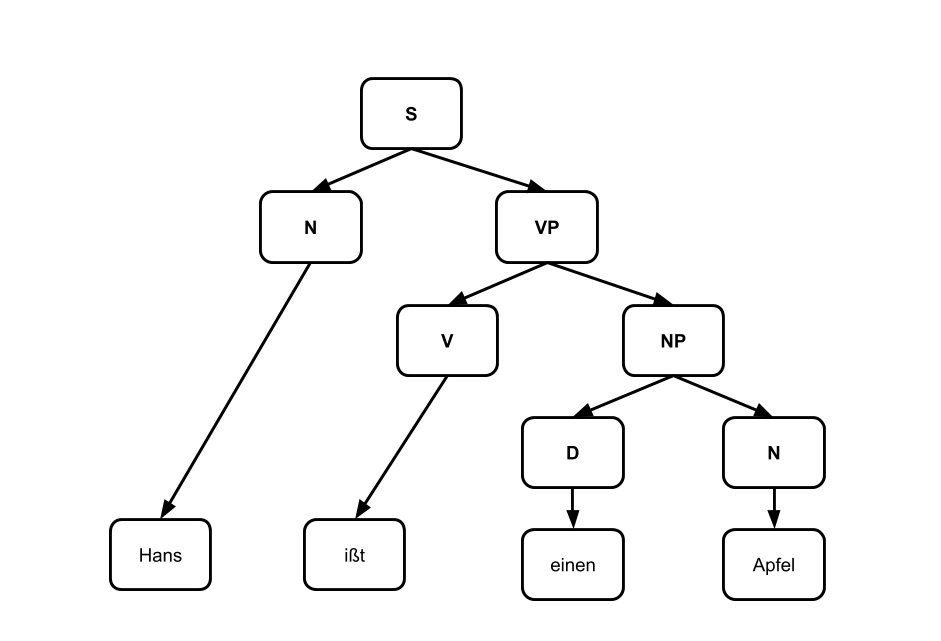
\includegraphics[width=\textwidth,height=8cm,keepaspectratio=true]
    {hans-eats-apples.png}
    \caption{
        An example parser tree
    }
    \label{fig:An example parser tree network}
\end{figure}

In this tree, the abbrevations S, D, N, V, NP and VP refers to sentence, determinant, noun, verb, noun-phrase and verb-phrase respectively. The words of the sentence are referred as leaf nodes of the tree: Hans, ißt, die and Äpfel. The parts of speech (POS) tags associated with the above words are noun(N), verb(V), determinant(D) and noun(N) respectively. These are referred as immediate parent of each word. The rest of nodes are formed out of parsing. From the diagram, it is clear that the sentence followed three rules:

S --> N VP \newline
VP --> V NP \newline
NP --> D N 

%Explanation about constituency parsing. How is it helpful
Jurafsky et al. \parencite{Jurafsky2008} in their 'Speech and Language processing' book stated that the parse tree is useful in many applications related to NLP. Infact they are directly useful in grammar checking in word processing systems; a sentence that cannot be parsed is supposed to have grammatical errors. Most of the times, it is also an important intermediate representation for the semantic analysis of sentence. Thus it plays an important role in application such as relation extraction, semantic role labeling \parencite{Gildea:2002:NPP:1073083.1073124}, question answering and paraphrase detection \parencite{Callison-Burch2010}.

%A brief history of constituency parsing. 
  %Different languages - different parsing rules
  %Handwritten rules to Machine learning based approach (statistical relationship)

%Penn Treebank dataset and SPMRL dataset  in state of parser in paper 'consituent parsing with a self attentive encoder'
% Applying state of the art approach to a new dataset - %Tübingen data
In this thesis, we will apply state of the art techniques to perform constituent parsing on German dataset released by University of Tübingen.

% ----------------------------------------------------------------------------
\pagebreak
\section{Related work}

% FIND PAPERS FOR FOLLOWING
% Handwritten rules for parsing 
% probabilisitic methods for context free grammars

In the past, handwritten grammars played a central role in parsing. Context free grammars (CFG) were used to model the rules and patterns of natural language. But given the complexity of a natural language, neither simple, broad-coverage grammar rules nor complex, constrained grammars were able to optimally accomodate sentences. A specific complex grammar with a lot of constraints was failing to parse a lot of sentences. At the same time, a simple and generic grammar was making it possible to have multiple ways of parsing even for a simple sentence. Statistical parsing systems offer a lot of possibilities of many rules to cope up with the flexibility of a language and at the same time has the predictive capabilities to figure out most likely parsing tree for a sentence. In order to build statistical parsing system, the need for a versatile dataset is very critical.

%There were considerable efforts put in by the research community to prepare large, standard and open datasets such as Wallstreet journal penn tree bank and SPGML, which is used as a standard benchmark to compare the algorithms. These datasets fuelled the research faster. 

Marcus et al.\parencite{Marcus1993} prepared Penn Tree Bank dataset for english language which consists of syntactic structures for sentences along with POS tags. It was revised multiple times and now it consists of more than 39,000 sentences with syntax trees and 7 millions of words with POS tags \parencite{Taylor2003}. These annotated information includes text from different sources such as IBM computer manuals, nursing notes, Wall Street Journal articles and transcribed telephone conversations. This served as a good corpus for building models to do parsing based on Machine Learning (ML). This lead to a empirical/data-driven approach to parsing than rule based approach. Some of the advantages of a treebank are reusability of lot of other subsystems such as POS taggers, parsers  and a standard way to evaluate multiple parsing systems. 

%CFG-PCFG- Chart based CKY algorithm 
%Lexicalization of production rules
%Sudviding the categories - split based on closed grammar, horizontal markovization (binarization) and vertical markovization (parent categories), combination of latent models

Probabilistic context free grammars (PCFG) contains a probability score assigned to each production rule. These probabilities are assigned based on various methods and the simplest of it is considering the statistical properties of word combinations. They help to quantify the likelihood of different possibilities of parsing a sentence. Chart based CKY algorithm is a bottom up parsing methodology which uses these probability scores to make decision about what combination of constituents are very likely. It only takes cubic time complexity rather than exponential by using dynamic programming techniques. 

The head word of a phrase gives a good representation of the phrase structure and meaning. 
PCFG parsing methods gives only 73 percent F1 score. Lexicalization of PCFG will create more rules pertaining to specific cases and the probability scores can be trained for each production rule. This indeed improves accuracy of parsing using Charniak method. But it increases production rules exponentially which results in sparseness. Kelin and Manning found that lexicalized PCFG does not capture lexical selection between content words but just basic grammatical features like verb form, verbal auxiliary, finiteness etc. This kind of splitting can be done horizontally while binarizing the tree and vertically by parent annotation \parencite{Gaddy2018}. It achieved 85.7percent F1 score and does not lead to too many production rules but at the same time captures the essence of context. Untill now the rules of grammar was handwritten which were picked carefully by experts. Petrov and Klein came up with a unsupervised ML approach which use base categories and learns subcategorizing and splitting using treebank data. They used expectation maximization (EM) algorithm, like Forward-Backward for HMMs but constrained by tree structure. 

On the other hand, neural networks have been raising and becoming a prominent architecture to build machine learning (ML) systems. They were giving state of the art results for many NLP applications. They are also used to develop a better alternative for representation of words or other features of text. 

% Recursive neural network
The constituent parsing of a given sentence involves outputting a tree which is fundamentally made of recursive structures of branches or merges of words or phrases. Socher et al. [\parencite*{RichardSocher2011}, \parencite*{Socher}, \parencite*{Sochera}] implemented a neural network based parsing which is specialized in learning recursive structures in a sentence and simultaneously learning compositional vectors for phrases. Their work achieved an accuracy of 90.4 F1 score and it is 20 percent faster than stanford factored parser. The system involves two bottom up parsing; the first parsing done by a base Probabilistic Context Free Grammar(PCFG) parser using CKY dynamic programming and select 200 best parses; the second pass is done by their best recursive neural network model with expensive matrix calculations on those 200 best results. 

%Encoder-Decoder artchitecture
%Encoder - FeedForward neural network, CNN, RNN , Bi-RNN,
%\parencite*{Vaswani2017}
%\parencite*{Stern2017}
%\parencite*{Gaddy2018}

Stern et al. \parencite*{Stern2017} implemented a minimum span neural network based constituency parser and achieved an accuracy of 91.79 F1 score on Penn Treebank dataset. They used an encoder-decoder architecture where in the encoder converts the input into a different reprsentation with context information and the decoder uses this augmented information to build the tree and get trained to become better. Bi-directional LSTM modules were used to encode the words in a sentence. This encoding gives out two vectors for each word containing the sentential context from left and right direction. This encoded output is used by two independent scoring systems; one to label the span and the other to choose the split. Their research work involved experimenting the above computed encoded output with chart-based bottom up and greedy top down parsing. Surprisingly the results of using top down with run time complexity O(n2) is as good as using bottom up approach where in a global optimized tree is chosen with run time complexity O(n3). The bottom up parsing was making decisions at every stage with the already computed values for whole tree beneath; whereas the top down parsing can refer to only local information. These results credit the ability of Bidirectional LSTM modules in capturing a lot of complex relations among words in a sentence. By using rich and expressive word vector representations, the encoding and decoding architectures are made simpler. 

%Encoder - self attention module
Kitaev et al. \parencite*{Kitaev2019} also implemented a encoder-decoder based neural network architecture for constituency parsing and they achieved state of the art accuracy of 95.13 F1 score on Penn Treebank dataset. Their parser also outperforms all the previous parsers on 8 of the 9 languages in SPMRL dataset. In this,, instead of LSTM modules, Attention modules \parencite*{Vaswani2017} are used. Attention modules are better in expressing how two sentences or inputs are relevant to each other by expressing them in a matrix with columns and rows as words/components of sentences/inputs of each. At the same time, attention modules can also be applied to a sentence itself to express which part of sentence is dependent on which other words. These capture the relationships of words in a sentence among themselves. Several self-attention modules are used in combination to encode the information and context in each sentence. The use of attention makes explicit the manner in which information is propagated between different locations in the sentence. A chart based decoder implemented by Stern et al. \parencite*{Stern2017} is used along with the modifications from Gaddy et al \parencite*{Gaddy2018}. They also found that positional information plays an very important role in parsing and inclusion of ELMo(Embeddings from Language Models) improved their accuracy by 3 percent. 

%Decoder - chartbased, greedy or beam search. top down and bottom up

% ----------------------------------------------------------------------------
\pagebreak
\section{Background Study}
In this thesis, we develop a neural network based constituent parser for german dataset released by Tübingen. The required information to understand different components of the proposed system is explained briefly in this section. 

Papers to write about:

Parser showdown at the wallstreet corral: An empirical investigation of error types

Parsing three german treebanks: Lexicalized and Unlexicalized Baselines


\subsection{Neural networks and its components}

Recently, neural networks have become the most popular approach for building machine learning systems. Neural networks compose many interconnected, fundamental, functional units called neurons. They are loosely inspired from the field of neuroscience. There are different ways by which these neurons can be connected with each other. That defines its ability to learn. 

Feed-forward neural network \parencite{Svozil1997} is a basic neural network architecture which arranges neurons in layers that reflect the flow of information. They are used to perform supervised machine learning where in label data regarding classification is mandatory. These networks should contain a input layer which takes in data and a output layer which represents prediction of classification. It can have one or many hidden layers and each neuron in one layer is connected with every other neuron in the subsequent layer as given in the Figure \ref{fig:Feed forward neural network}

A model, data, objective or loss function, and optimizer are important components of any machine learning approach.

,  to capabilities defines the architecture s of neural networks which vary mostly in how the neurons are connected. That defines the model

Each neuron in the network takes in multiple scalar inputs and gives out a scalar output. It uses parameters (weights and bias) to perform linear transformation of the input and most often applies non-linear function subsequntly.

\begin{figure}[htpb]
    \centering
    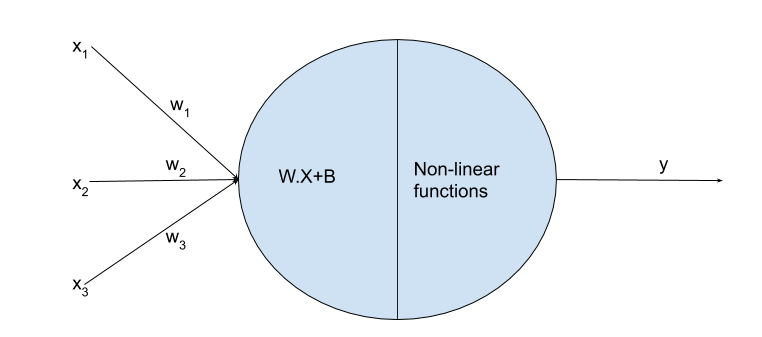
\includegraphics[width=\textwidth,height=8cm,keepaspectratio=true]
    {single-neuron.png}
    \caption{
        Single Neuron
    }
    \label{fig:single_neuron}
\end{figure}

 to linearly transform the valuemultiplies each input by a weight and then sums them, adds the result with a bias, applies a non-linear function at the end, which gives out a scalar output. 



There are different architectures of neural networks which vary mostly in how the neurons are connected to each other and how the weights are managed. Feed-forward neural networks \parencite{Svozil1997} can have multiple layers and each neuron in one layer is connected with every other neuron in the subsequent layer as given in the Figure \ref{fig:Feed forward neural network}

\begin{figure}[htpb]
    \centering
    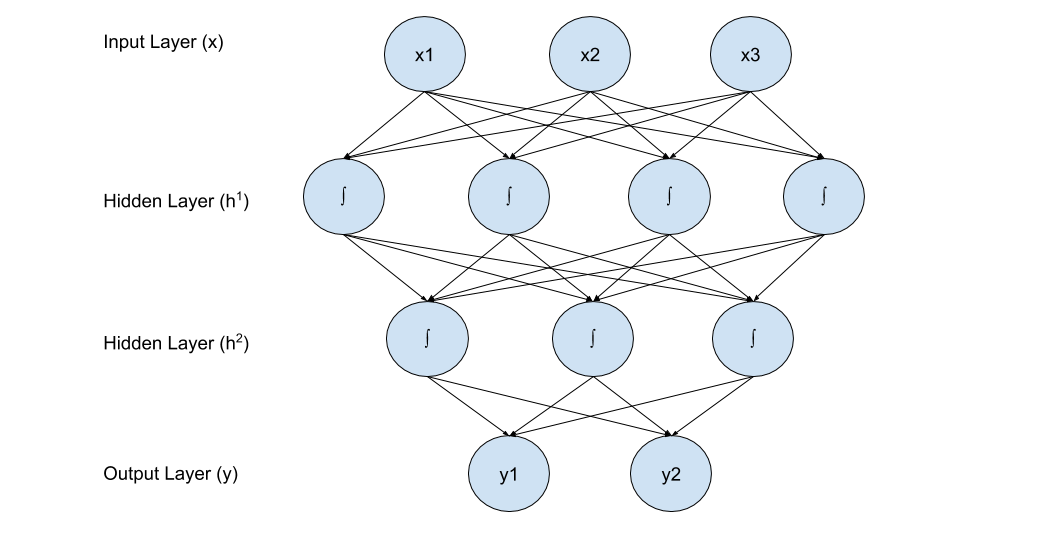
\includegraphics[width=\textwidth,height=8cm,keepaspectratio=true]
    {feed-forward-neural-network.png}
    \caption{
        A Feed-Forward neural network.
    }
    \label{fig:Feed forward neural network}
\end{figure}

There are 4 layers in figure \ref{fig:Feed forward neural network}. Each circle is a neuron with incoming lines as inputs and outgoing lines as outputs to the next layer. Each line carries a weight and the input layer has no weights since it has no incoming lines. The input layer consists of 3 neurons and the extracted features of raw data will be sent through these neurons. The first hidden layer consists of 4 neurons, of which each neuron takes 3 inputs from input layer. Each input to the neuron in first hidden layer is multiplied by a unique weight variable and added together.  Finally, the output is added with a bias variable and will be passed to a non-linear activation function as shown in equation \ref{equ: feed forward hidden layer}. The same process is carried out for the second hidden layer except that it has 3 neurons and each neuron will take 4 inputs from the first hidden layer. The output layer consists of 2 neurons and each will take 3 inputs from second hidden layer as shown in equation \ref{equ: feed forward output layer}.

\begin{equation} \label{equ: feed forward hidden layer}
h^1 = g^1(xW^1 + b^1)
\end{equation}

\begin{equation}
h^2 = g^2(h^1W^2 + b^2)
\end{equation}

\begin{equation} \label{equ: feed forward output layer}
\mathrm{NN_{MLP2}}(x) = y = g^3(h^2W^3 + b^3)
\end{equation}
\begin{align*}
x \in \mathbb{R}^{d_{in}}, y \in \mathbb{R}^{d_{out}} \\
W^1 \in \mathbb{R}^{d_{in} \times d_1}, b^1 \in \mathbb{R}^{d_1}, h1 \in \mathbb{R}^{d_{1}} \\
W^2 \in \mathbb{R}^{d_1 \times d_2}, b^2 \in \mathbb{R}^{d_2}, h2 \in \mathbb{R}^{d_{2}}\\
W^3 \in \mathbb{R}^{d_2 \times d_\mathrm{out}}, b^3 \in \mathbb{R}^{d_{out}}
\end{align*}

Here $\mathbf{W^1, W^2, W^3}$,  and $\mathbf{b^1}$, $\mathbf{b^2}$ and $\mathbf{b^3}$ are matrices and bias vectors for first, second and third linear transforms, respectively. The functions $g^1$, $g^2$ and $g^3$ are activation functions and they are almost always non-linear. With respect to figure~\ref{fig:Feed forward neural network}, the values of $d_\mathrm{in}$, $d_{1}$, $d_{2}$ and $d_\mathrm{out}$ are 3, 4, 3, and 2, respectively. 

The activation functions help the neural network models to approximate any nonlinear function. Different activation functions pose different advantages. Some popular activation functions are sigmoid, hyperbolic tangent and rectifiers \parencite{Goldberg2016}:

\begin{enumerate}

\item The sigmoid activation function is a S-shaped function which transforms any value into the range between $0$ and $1$.  
\begin{align*}
\sigma (x) = \frac{1}{1 + e^{-x}}
\end{align*}

\item The hyperbolic tangent function is also a S-shaped function, but it transforms any value into the range between $-1$ and $1$.
\begin{align*}
\tanh (x) = \frac{e^{2x}-1}{e^{2x}+1}
\end{align*}

\item The rectifier activation function clips values lesser than $0$
\begin{align*}
\mathrm{ReLU}(x) = \mathrm{max}(0,x)
\end{align*}

\end{enumerate}

The sigmoid activation function is not used in internal layers of neural networks since other functions have been giving better results empirically. The rectifier activation function is commonly used since it performs faster and better than sigmoid and hyperbolic tangent functions. Instead of an activation function, the function in output layer $g^3$ can be a transformation function such as softmax to convert values to represent a discrete probability distribution. Each of the converted values will be between $0$ and $1$ and sum of all of them will be $1$.

\begin{align*}
y = \begin{bmatrix} y_1 & y_2 & \dots & y_k \end{bmatrix} \\
s_i = \mathrm{softmax(y_i)} = \frac{e^{y_i}}{(\sum_{j=1}^ke^{y_j})}
\end{align*}

\subsection{Training a neural network}

Training is an essential part of learning and like many supervised algorithms, a loss function is used to compute the error for the predicted output against the actual output. The gradient of the errors is calculated with respect to each weight and bias variable by propagating backward using chain rule of differentiation. The values of the weights and bias are adjusted with respect to the gradient and a learning parameter. Typically a random batch of inputs is selected and a forward pass is carried out which involves multiplying weights, adding bias and applying an activation function to predict outputs. The average loss is computed for that batch and the parameters are adjusted accordingly. This optimization technique is called stochastic gradient descent \parencite{Bottou2012}. A number of extensions exists, such as Nesterov Momentum \parencite{Sutskever2013} or AdaGrad \parencite{Duchi2011}. Some loss functions that exist are hinge loss (binary and multiclass), log loss and categorical cross-entropy loss \parencite{Goldberg2016}. 

%\begin{align*}
%L_{hinge(binary)}(\hat{y},y) = max(0,1-y.\hat{y})
%\end{align*}

The categorical cross-entropy loss is used when predicted output refers to a probability distribution. This is typically achieved by using a softmax activation function in the output layer. Let $y = y^{1}, y^{2}, \dots, y^{n}$ be representing the target multinomial distribution over the labels $1,2,\dots,n$ and let $ \hat{y} = \hat{y}_{1},\hat{y}_{2},\dots,\hat{y}_{n}$ be the network's output which is transformed by a softmax function. The categorical cross-entropy loss measures the difference between the true label distribution $y$ and the predicted label distribution $\hat{y}$. 
\begin{align*}
L_\mathrm{cross-entropy}(\hat{y},y) = -\sum_iy_i \cdot \log(\hat{y_i})
\end{align*}

For hard classification, $y$ is a one-hot vector representing the true class. Here $t$ is the correct class assignment. Training will attempt to set the correct class $t$ to 1 which inturn will decrease the other class assignment to 0.
\begin{align*}
L_{\mathrm{cross-entropy(hard classification)}}(\hat{y},y) = -\log(\hat{y_t})
\end{align*}

The overfitting in neural networks will cause the trained system to perform well only for trained data but not on the test data. This can be minimized by using regularization techniques such as $L_2$ regularization and dropout \parencite{Hinton2012}. $L_2$ regularization works by adding a penalty term equal to sum of the squares of all the parameters in the network to the loss function which is being minimized. Dropout, instead, works by randomly ignoring half of the neurons in every layer and corrects the error only using the parameters of other half of neurons. This helps to prevent the network from relying on only specific weights.

\subsection{Neural networks for text data}

In case of text data, the input is sequential and of unknown length, where the ordering of words is important. Techniques such as continuous bag of words \parencite{DBLP:journals/corr/abs-1301-3781} can be used with feed-forward networks to convert sequential input into fixed length vectors but it will discard the order of words. Convolutional neural networks (CNN) \parencite{Bengio1997} are good at capturing the local characteristics of data irrespective of its position. In this, a nonlinear function is applied to every $k$-word sliding window and captures the important characteristics of the word in that window. All the important characteristics from each window are combined by either taking maximum or average value from each window. This captures the important characteristics of a sentence irrespective of its location. However, because of the nature of CNNs they fail to recognize patterns that are far apart in the sequence.

Recurrent neural networks (RNN) accept sequential inputs and are often able to extract patterns over long distances \parencite{Elman}. A RNN takes input as an ordered list of input vectors $\mathrm{\mathbf{x_1},\dots,\mathbf{x_n}}$ with initial state vector $\mathbf{h_0}$ and returns an ordered list of state vectors $\mathrm{\mathbf{h_1},\dots,\mathbf{h_n}}$ as well as an ordered list of output vectors $\mathrm{\mathbf{o_1},\dots,\mathbf{o_n}}$. At time step $t$, a RNN takes as input a state vector $\mathbf{h_{t-1}}$, an input vector $\mathbf{x_{t}}$ and outputs a new state vector $\mathbf{h_{t}}$ as shown in figure \ref{fig:A basic RNN architecture}. The outputted state vector is used as input state vector at the next time step. The same weights for input, state, and output vectors are used in each time step.  

%RNN - architecture, how does it support the sequence, (Elman, 1990) 
%Back Propagation through time (BPTT) - (Werbos, 1990) \parencite{Werbos1990}
%Long distance dependencies - LSTM and GRU (Hochreiter and Schmidhuber 1997) and (Cho et al.)
%(did not find the citation for GRU) \parencite{Hochreiter1997}
%Recursive Neural Networks - for syntactic structure (trees ) (pollack 1990; socher, manning and ng 2010) \parencite{Pollack1990} \parencite{Socher}

\begin{figure}[htpb!]
    \centering
    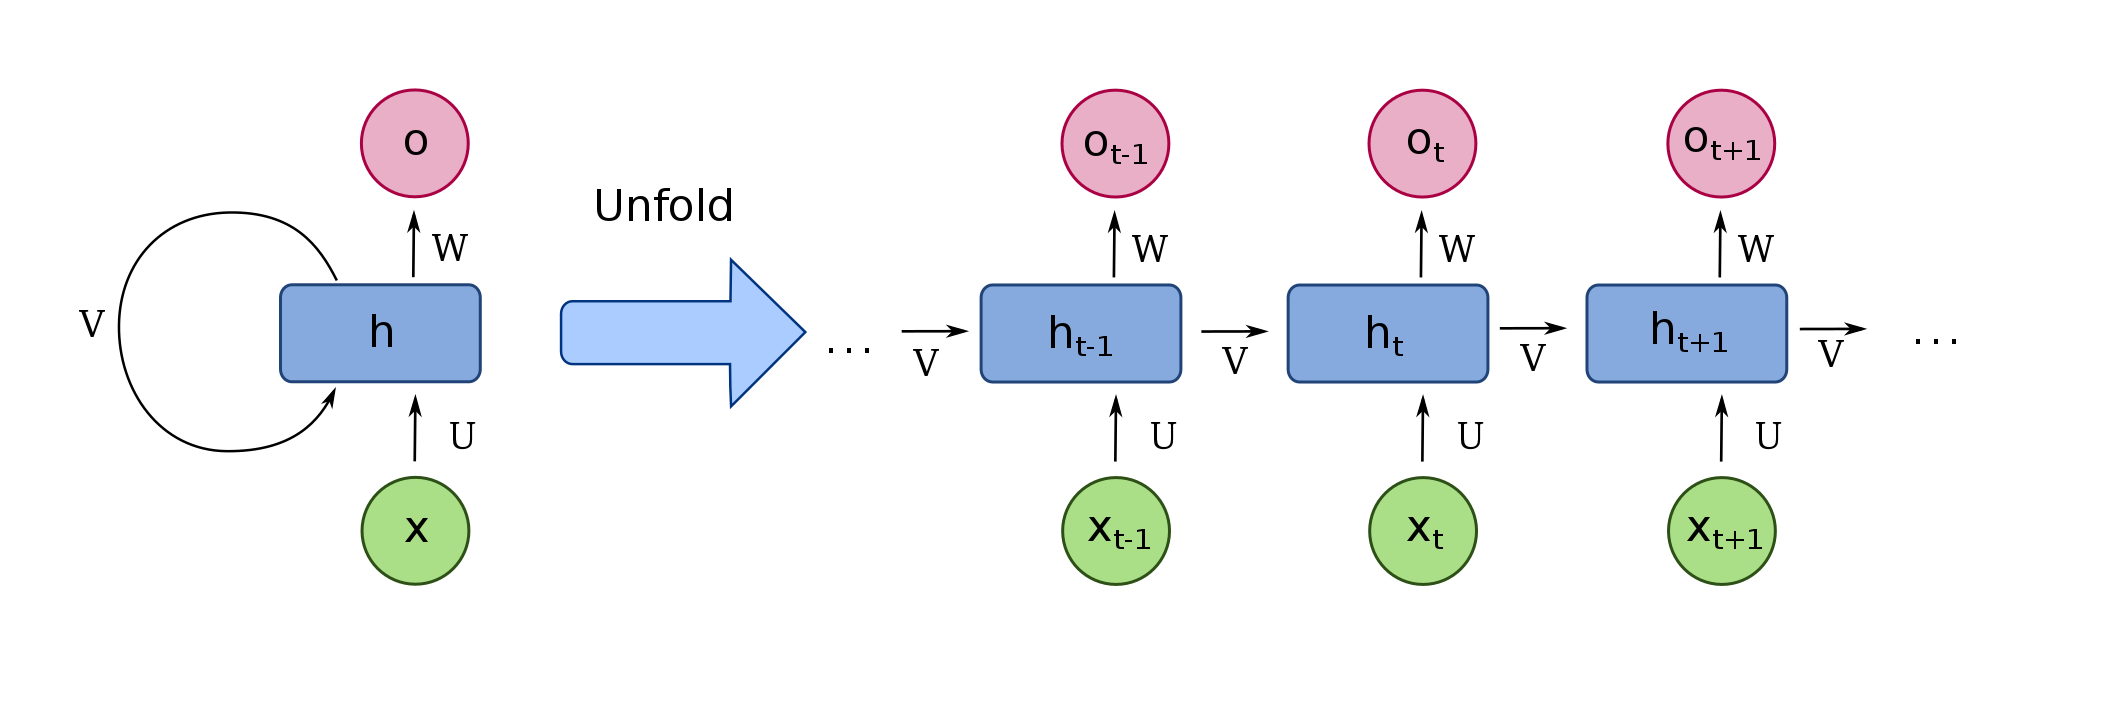
\includegraphics[width=\textwidth,height=6cm,keepaspectratio=true]
    {Recurrent_neural_network_unfold.png}
    \caption{
        A basic example of RNN architecture \parencite{WikipediaEN_RNN_unfold}.
    }
    \label{fig:A basic RNN architecture}
\end{figure}

\begin{align*}
\mathrm{RNN}(h_0,x_{1:n}) = h_{1:n}, o_{1:n} \\
h_i = g^1(h_{i-1}V + x_iU + b^1) \\
o_i = g^2(h_iW + b^2) 
\end{align*}

\begin{align*}
x_i \in \mathbb{R}^{d_x}, U \in \mathbb{R}^{d_x \times d_h} \\
h_i \in \mathbb{R}^{d_h}, V \in \mathbb{R}^{d_h \times d_h}, b^1 \in \mathbb{R}^{d_h} \\
o_i \in \mathbb{R}^{d_o}, W \in \mathbb{R}^{d_h \times d_o}, b^2 \in \mathbb{R}^{d_o}
\end{align*}

Here the functions $g^{1}$ and $g^{2}$ are non-linear activation functions; $\mathbf{W}$, $\mathbf{V}$, and $\mathbf{U}$ are weight matrices and $\mathbf{b^{1}}$, $\mathbf{b^{2}}$ are bias vectors. 

To train a RNN, the network is unrolled for a given input sequence and the loss function is used to compute the gradient of error with respect to parameters involved in every time step by propagating backward through time. After that, the parameters are adjusted to reduce the error in prediction \parencite{Werbos1990}. While training RNNs, a common problem that especially occurs with long input sentences is that the error gradients might vanish (become too close to zero) or explode (become too large) which results in numerical instability during the backpropagation step. The gradient explosion can be handled by clipping a given gradient when it goes beyond the threshold. LSTM networks \parencite{Hochreiter1997} solve the vanishing gradient problem by introducing memory cells which are controlled by gating components. These gating components decide at each time step, what parts of the hidden state should be forgotten and what parts of new input should be included into the memory cells. These memory cells are involved in the computation of hidden states, which in turn are used to compute the output states. This technique has been shown to provide good results in practice, in capturing the dependency between words even though separated by a long distance.

%\begin{align*} \label{lstm_equation}
%s_j = R_{LSTM}(s_{j-1},x_j) = [c_j;h_j] \\
%c_j = c_{j-1} \odot f + g \odot i \\
%h_j = tanh(c_j) \odot o \\
%i = \sigma(x_jW^{xi} + h_{j-1} W^{hi}) \\
%f = \sigma(x_jW^{xf} + h_{j-1} W^{hf}) \\
%o = \sigma(x_jW^{xo} + h_{j-1} W^{ho}) \\
%g = \sigma(x_jW^{xg} + h_{j-1} W^{hg}) \\
%y_j = O_{LSTM}(s_j) = h_j \\
%s_j \in \mathbb{R}^{2.d_h},   x_i \in \mathbb{R}^{d_x},  c_j,h_j,i,f,o,g \in \mathbb{R}^d_h, \\
%W^{xo} \in \mathbb{R}^{d_x*d_h},  W^{ho} \in \mathbb{R}^{d_h*d_h}
%\end{align*}
%Here the symbol $\odot$ denotes component wise product. The LSTM uses 3 gating components such as input gate (i), forgot gate (f) and output gate (o) respectively. They contain a sigmoid function to convert the values between 0 and 1 which is used to decide how much to keep. The memory cell state c\textsubscript{j} is obtained by controlling the previous memory cell state with forgot gate and the new input state (g) with input gate. The obtained memory cell state is controlled by output gate to get the hidden state h\textsubscript{j}.

\subsection{Neural networks for parsing }

A RNN computes the state of current word $\mathbf{x_{i}}$ only based on the words in the past, i.e. $\mathrm{\mathbf{x_1},\dots,\mathbf{x_{i-1}}}$. However, the following words $\mathrm{\mathbf{x_{i+1}},\dots,\mathbf{x_{n}}}$ will also be useful in computing the hidden state regarding the current word. The Bidirectional RNN (biRNN) (Schuster and Paliwal, 1997) solves the problem by having two different RNNs. The first RNN is fed with the input sequence $\mathrm{\mathbf{x_{1}},\dots,\mathbf{x_{n}}}$ and the second RNN is fed with input sequence in reverse. The hidden state representation $\mathbf{h_{i}}$ is then composed of both the forward and backward states. Each state representation consists of the token information along with sentential context from both directions which has shown better results than classical uni-directional RNNs in practice.

The mentioned approaches take only Wikipedia sentence as an input. This can be extended further by feeding information which gives context about the input sentence. This extra information might enable the system to perform efficiently in classifying whether a news item is fake or not. Attention mechanism in neural networks is used to take two inputs and convert it into one common representation. This is done by configuring the level of attention that needs to be given to different parts of each input and combine them to form a single output. Most often the inputs will be matrices and the output will be a vector. Bidirectional RNNs can be used to convert both input and context information into matrices. The fixed output vector is then fed into a deep feed-forward neural network to predict a class. Attention mechanism with RNN gives state of the art results in many NLP applications such as Natural Language Inference \parencite{Parikh2016}, Machine Translation \parencite{Bahdanau2014} and Document classification \parencite{Yang2016}.

\subsection{Self Attention}


\pagebreak
\section{Approach}  

In this thesis work, deep learning techniques are used to develop constituent parser for german language. This section explains in detail about the architecture used and different components included in it. In this approach, the german dataset released by by Tübingen is used to train the model effectively.

\subsection{Research Questions}

Through this work, the research questions that would be addressed are:
\begin{enumerate}
\item How well the self attention based modules of neural network are effective in capturing constituency grammar of german language? 
\item How efficient the model can be improved by using only the tree dataset? This means no other external data directly or indirectly will be utilised. 
\item How efficient the model can be improved using Transfer learning which involves pre-trained deep learning systems using external data such as German Wikipedia?
\item What components of ELMo are useful for building an efficient model? ELMo uses combination of three layers of its output data by computing a weighted sum of each layer. The research also involves in figuring out which layer or what combination of layers output is pertinent to this particular task of developing consituent parser.
\end{enumerate}

\subsection{Model}

The models are highly inspired from the works of Kitaev et al. \parencite*{Kitaev2019}, which involves an encoder-decoder architecture as shown in figure \ref{fig:broad_architecture}:

\begin{figure}[htpb]
    \centering
    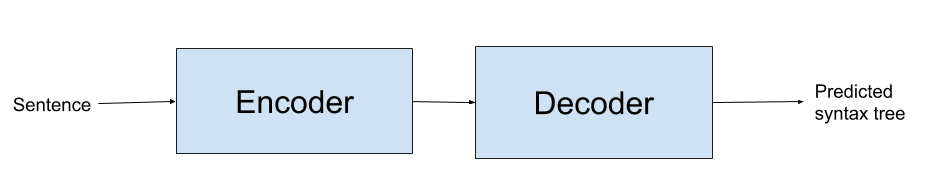
\includegraphics[width=\textwidth,height=8cm,keepaspectratio=true]
    {encoder-decoder.png}
    \caption{
        Broad Architecture
    }
    \label{fig:broad_architecture}
\end{figure}

The input to this system is a german sentence and the output is a predicted syntax tree of that particular sentence. The encoder takes in input sentence and does processing to convert it into a convenient, rich and versatile representation. This representation embodies information for each word with sub-word patterns as well as the context of the whole sentence. The encoded output is then fed into a decoder which outputs syntax tree. The building of syntax tree is seen as a continuous iteration of merging of certain subsequent words or merges that already happened in hierarchy. The decoder method involves steps to figure out what combination of merges are the best to build a good syntax tree.

The training of deep learning system involves a objective function to compare the prediction against golden output to allow fine tuning of different components of model using backward propagation of gradients of error. In this context, the predicted best possible syntax tree is compared against the golden tree and the parameters involved in the encoder section is updated accordingly to yield the best syntax tree next time. 

There are many ways by which the encoder and decoder components can be modeled. But in this approach, the encoder and decoder components are fixed and only the representation of sentences is varied to a certain degree. The encoder module is inspired from a state of art transformer neural network which predominantly uses self-attention modules, whereas the decoder module uses CKY approach to build the syntax tree. Sentences are represented using character embeddings and different word embeddings. In addition to words, position information of words are also used separately. The system does not use any other pre-processed information such as Parts Of Speech (POS) obtained by external tagger system as in old parsing methods.

\subsubsection{Encoder}

The purpose of the encoder, in this context, is to represent a sentence into a rich format which encompasses the sub-word patterns as well as the overall context of a sentence. This is achieved through a multi-layered, multi-head attention modules backed up with feed-forward networks as shown in the figure \ref{fig:encoder_module}

\begin{figure}[htpb]
    \centering
    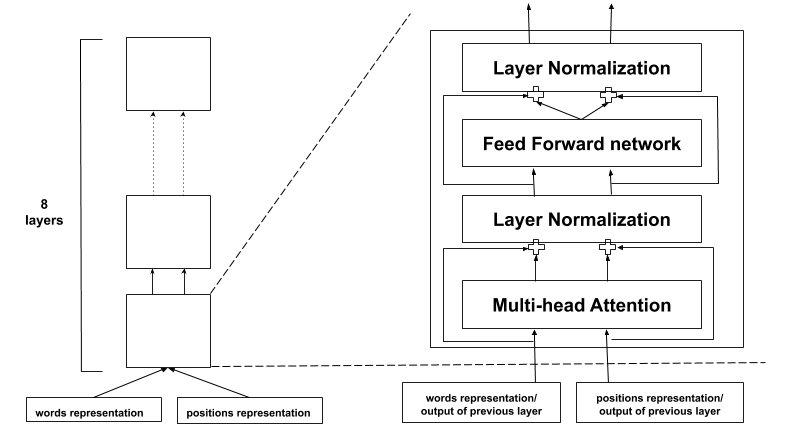
\includegraphics[width=\textwidth,height=15cm,keepaspectratio=true]
    {encoder.png}
    \caption{
        Encoder module
    }
    \label{fig:encoder_module}
\end{figure}

The input to this system is passed through 8 identical layers made up of multi-head self-attention mechanism modules sequentially. The output of the first layer is passed as input to the second layer. At each layer, the representation of a sentence is expected to improve gradually. A Multi-head attention uses 8 single heads, whereas each one allows every word in a sentence to gather information from one word in the same sentence. This brings out a matrix of information regarding what words attend to or obtain information from what other words in a sentence. This is applied not only to words but also to positions separately. Kitaev et al. \parencite*{Kitaev2019} shown in their work that separating words and positions for building constituent parser improved the results by 0.5 F1 score. And also that, position attention contributes more than content attention by 18 F1 score. Hence the position attention is used separately. 

The output of Multi-head attention module is then passed to Layer Normalization by mixing with residual component of input. The Normalization of intermediate result along with objective function will help the gradient based optimizer to arrive the best values quickly. A Feed-forward network at this juncture helps to look for patterns among the multiple attention representation of words in a sentence and also to map the intermediate result dimension space to be compatible with inputs and outputs of each layer.  

The dimensionality of representation, inputs and outputs of each layer are the same. A total of 1024 neurons are used to represent and it is split half and used by word and position related functions respectively. 


The figure \ref{fig:single_attention_head} shows the outline of what happens inside a single attention head:

\begin{figure}[htpb]
    \centering
    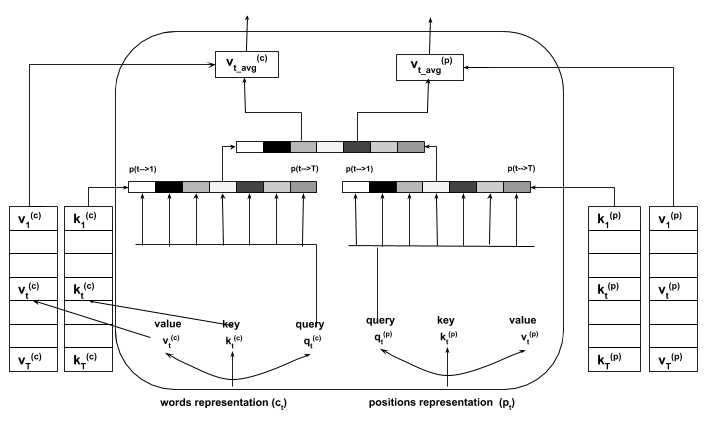
\includegraphics[width=\textwidth,height=10cm,keepaspectratio=true]
    {single-head-attention.png}
    \caption{
        Single attention head
    }
    \label{fig:single_attention_head}
\end{figure}


Each word or position representation is transformed into 3 vectors such as key $(k_t)$,  value $(v_t)$ and query $(q_t)$ with lesser dimensions $(d_k)$. This is done by using separate trainable parameters for word and position representation as well as for the above three entities. For example, the parameters for key transformation for both word and position representation are $W^{c}_K$ and $W^{p}_K$ respectively.

The attention of a word i to a word j in a sentence is then calculated as 
$ p(i\rightarrow{}j) \propto exp(\dfrac{q^{(c)}_i.k^{(c)}_j}{sqrt(d_k)}) $. In words, it is essentially a normalized dot product of respective query and key vectors. The weighted average of all values to form a average vector $\hat{v}_i = \sum_k p(i\rightarrow{}k)v_k$ represents the new value vector for word i which includes all the attention that it has on all the words in the sentence. 

The following set of equations reveal overall functionality of single attention head in mathematical terms. The query, key and value vectors are computed by respective weight parameters against the word representation. The output of this is a vector for each and every word. A matrix containing all the vectors concatenated represents the overall sentence and they are shown as $Q_p$, $K_p$, and $V_p$ respectively. The softmax function models the probability distribution of the dot product of query and key matrix. The dot product with value matrix computes the weighted average and it is transformed by $W^{(c)}_O$ matrix to align with other output dimensions.
\begin{align*}
q^{(c)}_t = W^{(c)}_Q c_t, k^{(c)}_t = W^{(c)}_K c_t, v^{(c)}_t = W^{(c)}_V c_t \\
SingleHead(C) = \left[softmax\left(\dfrac{Q_cK^T_c}{\sqrt{d_k}}\right) V_c\right] W^{(c)}_O \\
where\ Q_c = C{}W^{(c)}_Q; K_c = C{}W^{(c)}_K; V_c = C{}W^{(c)}_V  
\end{align*}

Similarly for position representation, the following equations convey single head functionality. Different set of trainable parameters are used to get the final output.
\begin{align*}
SingleHead(P) = \left[softmax\left(\dfrac{Q_pK^T_p}{\sqrt{d_k}}\right) V_p\right] W^{(p)}_O \\
where\ Q_p = P{}W^{(p)}_Q; K_p = P{}W^{(p)}_K; V_p = P{}W^{(p)}_V
\end{align*}

The output of single attention head is concatenated as shown in the figure \ref{fig:multi_head_attention_module}
\begin{figure}[htpb]
    \centering
    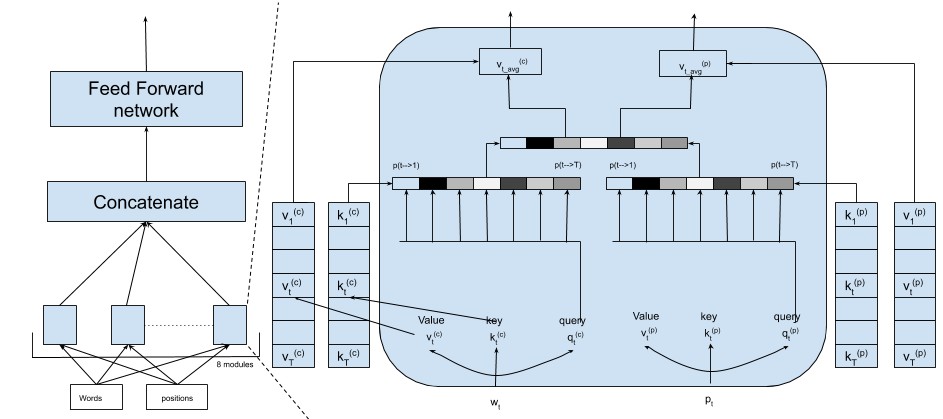
\includegraphics[width=\textwidth,height=10cm,keepaspectratio=true]
    {multi-head-attention.png}
    \caption{
        Mult-head attention module
    }
    \label{fig:multi_head_attention_module}
\end{figure}

The concatenated output fed through feed-forward to derive the patterns across multiple attentions in a sentence. These are then fed to Layer Normalization block as shown in the figure \ref{fig:encoder_module}.

\subsubsection{Decoder}
As shown in the section, the chart parser is inspired from the works of Stern et al. and Gaddy et al.

\subsubsection{Objective function}
max - margin, scoring . how does it work with CKY parsing and decoding

\subsection{Experiments}

The experiments are different for different pursuit of research questions. But the findings of one research is used in the subsequent researches. 

\subsubsection{For research question1:}
The first research question address how effectively self-attention module can be utilized to maximize the optimal building of constituent parser. The following points cover the idea of experiments that will be conducted for this scenario:
\begin{enumerate}
\item The first parameter that controls the self-attention module is the number of self-attention heads $(n_h)$. This helps the system to let the words to gather information from multiple locations in the same sentence. 
\item The next parameter which influences the output is the number of identical layers $(n_l)$ that are stacked above each other. It helps the system to draw generalized or abstract or deep patterns from the primitive low level patterns already computed. 
\item The internal dimension parameter for key, value and query attributes. This is used in conjunction with number of self-attention heads. In this approach, this is assigned with a fixed value 64 and the first parameter is changed. This particular value is taken from the research carried out by Kitaev et al. \parencite*{Kitaev2019}
\end{enumerate}

The assumption is that the more the value the better the result will be. But after some point, the rate of returns will be diminishing. A range of values are fixed both the parameters and experiments will be conducted. The result metric will be computed and tabulated as show below:

\begin{table}[h!]
  \begin{center}
    \begin{tabular}{c|c|c|c|c|c|c} 
      $n_l/n_h$ & $1$ & $3$ & $5$ & $8$ & $10$\\
      \hline
      1 & & & & & & \\
      \hline
      3 & & & & & \\
      \hline
      5 & & & & & \\
      \hline
      8 & & & & & \\
      \hline
      10 & & & & & \\
    \end{tabular}
    \caption{Parameters range table for Research question 1}
    \label{tab:research_question1_table1}

  \end{center}
\end{table}

Ideally all the variables should be changed and result metric should be computed and tabulated. The pair of $(n_l,n_h)$ values for which the resultant metric value is high, will be chosen as an ideal combination.But given the limiation on computation power and also the time, instead of choosing a classical Grid search which covers all the 25 combinations, random set of pairs will be chosen. In addition to that, Kitaev et al. from their research, chose value to be 8 after hyper tuning for both $n_l$ and $n_h$ respectively. Given these conditions, at the max, 5 experiments will be conducted which will be around the value 8.

\subsubsection{For research question2:}

Second research question - what is the most efficient constituent parser that can be built only with training data

representation embeddings matrix - integer to vector

1) character embeddings - . Bidirectional LSTM character - outputs concatenate. Word vectors are formed on the fly 
2) word embeddings - training
3) character + word embeddings

highest value of result metric

\subsubsection{For research question3:}

Third research question - Usage of ELMo. what components of it is the best to be used 

representation embeddings matrix - integer to vector

1) only the first layer
2) Second layer - syntactic relations are captured. 
3) Third layer - semantic. must have context
4) All layers combined with training

result metric

\pagebreak
\section{Evaluation}

Constituent parsing evaluation. The test data should be different from the training or validation data which is used by the system. 

\subsection{Datasets}

Tübingen dataset - write about history, coverage, versatility, who and what system have used it 


\subsection{Metrics}

Tree score
The following factors are used to compare the baseline with the improved system
\begin{enumerate}
\item how well constituent parsing of test dataset works out
\item F1 score
\end{enumerate}

The quality of the system can be measured by metrics such as Precision, Recall, F1 measure, and Accuracy. The F1 measure is preferred since it includes both false positive and false negatives. In this master thesis, the focus is mainly on improving the accuracy of the system and the speed of the system can be improved by using good hardware.

\pagebreak
\section{Implementation}

Implementation: Tensorflow, spacy 

CUDA drivers, GPU
Implementation: Pytorch, Spacy
Spacy and python libraries - pre-processing, there was some problem with the dataset and we removed it

Code inspiration - share the github link
Elmo - pre-trained dataset. download from a website - share it

Docker implementation- overnight runs 

%Recurrent neural networks will be used in this master thesis extensively since they perform well with sequential data. TensorFlow\footnote{https://www.tensorflow.org/} is a python library for building intensive numerical computation applications and deploy them in multiple platforms such as CPU and GPU. TensorFlow has built-in libraries to develop different neural network architectures. Wikipedia consists of a lot of articles; each article consists of a lot of sentences. Each sentence will be fed as input to the neural network.
%---------------
%An advanced RNN architecture takes in either one or two inputs such as sentence in Wikipedia and context information. The context can be empty. The system processes the input and produces a binary output representing true or fake news. The outputs would contain a probability distribution of how likely it is true or fake news.

%The inputs, in general, will be pre-processed to extract tokens, remove common words such as articles, prepositions and perform lemmatization which is converting the words to its root form. Low dimensional and dense word embeddings will be used to represent the inputs instead of one hot vectors. Already available word embeddings such as Word2vec \parencite{Mikolov2013} and GloVe\footnote{https://nlp.stanford.edu/projects/glove/} will be used to represent the inputs.

%The dataset will be split and used for training, validation, and testing of the system. A general rule of thumb is to divide the dataset into 60-20-20 for training, validation, and testing respectively. But if the datasets are in order of millions then it is good enough to have approximately 10000 entries each for validation and testing. The validation dataset is used to try out different hyper-parameter configurations and select the optimal values for each. The hyper-parameters of the advanced neural network system that will be configured are number of layers, learning parameter, batch size, activation functions and epoch number(number of times the training dataset should be iterated).

% Background Knowledge: Wikidata or BabelNet (knowledge graphs), http://babelfy.org/ for entity resolution

%The proposed methods involve modeling the content of Wikipedia in different ways such that the system can understand it better. These procedures are completely automatic in building the training examples and none of the features will be manually crafted. The different configurations of the system along with unique methods in constructing the training data is expected to understand Wikipedia better and the fake news detection can be carried out in a platform agnostic manner. 

% ----------------------------------------------------------------------------



\pagebreak
\section{Analysis}
Research question by question

Self - attention module - how does it capture context 
\pagebreak
\section{Conclusion}
% ----------------------------------------------------------------------------

Self attention
char encoding
char encoding + word embeddings

elmo embeddings
 

% ----------------------------------------------------------------------------

% ----------------------------------------------------------------------------
\newpage
\printbibliography
%\bibliography{bib.bib}
\newpage
% ----------------------------------------------------------------------------
\section{Signatures}

\vspace{3cm}
\begin{tabular}{ccc}
  --------------------------------------------------- &  & \\
  \myName{} &  &  \\ \vspace{3cm}
   &  &   \\
  --------------------------------------------------- &  & ---------------------------------------------------\\
  \secondSupervisor{} &  & \supervisor{}  \\ \vspace{3cm}
   &  &   \\
\end{tabular}

\newpage
% ----------------------------------------------------------------------------
\section{Declaration of Authorship}
I hereby declare that the thesis submitted is my own unaided work. All direct or indirect sources used are acknowledged as references.

I am aware that the thesis in digital form can be examined for the use of unauthorized aid and in order to determine whether the thesis as a whole or parts incorporated in it may be deemed as plagiarism. For the comparison of my work with existing sources I agree that it shall be entered in a database where it shall also remain after examination, to enable comparison with future theses submitted. Further rights of reproduction and usage, however, are not granted here.

This paper was not previously presented to another examination board and has not been published.

\vspace{3cm}
\begin{tabular}{ccc}

  Koblenz, on \today &  &  \\
     &  & ---------------------------------------------------\\
   &  & \myName{}  \\
\end{tabular}



\end{document}









